\pagebreak
%\clearpage

\thispagestyle{empty}
\ThisTileWallPaper{1.45\paperwidth}{1.0\paperheight}{images/fret}
%\begin{center}
%{\Large \textbf{}}
%\end{center}

\addtolength{\wpXoffset}{-4.5cm}

\justify

%{\LARGE
%
%\color{white}{Ce rapport propose une analyse stratégique du fret aérien suiviant le modèle de Porter.}
%}

%\begin{figure}[!h]
%	\begin{center}
%		\label{}
%		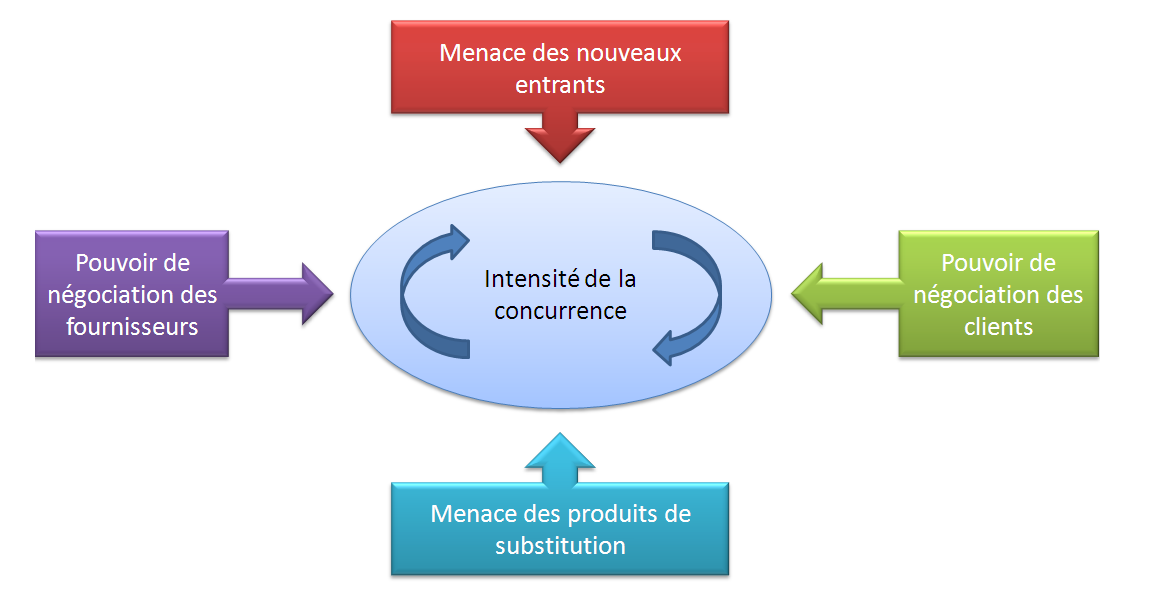
\includegraphics[scale=0.4]{images/porter/porter_2}
%	\end{center}
%\end{figure}



%\begin{tikzpicture}[remember picture, overlay]
%\begin{scope}[shift={(current page.south west)},shift={(1,1)},scale=1]
%\shade[ball color=blue,opacity=.6] (0,0) circle (10ex);
%\shade[ball color=blue,opacity=.8] (1.7,1) circle (5ex);
%\shade[ball color=blue,opacity=.8] (1.5,3) circle (2ex);
%\shade[ball color=blue,opacity=.5] (-0.5,3) circle (1ex);
%\shade[ball color=blue,opacity=.8] (1,4) circle (1ex);
%\shade[ball color=blue,opacity=.6] (3.5,2.5) circle (2ex);
%\shade[ball color=blue,opacity=.8] (2.5,4.5) circle (4ex);
%\shade[ball color=blue,opacity=.5] (3,4) circle (3ex);
%\shade[ball color=blue,opacity=.8] (4.5,4.5) circle (3ex);
%\shade[ball color=blue,opacity=.5] (5.1,4.7) circle (2ex);
%\shade[ball color=blue,opacity=.8] (5,6) circle (1.5ex);
%\shade[ball color=blue,opacity=.6] (3.5,5.5) circle (2ex);
%\shade[ball color=blue,opacity=.8] (5,3) circle (1ex);
%\end{scope}
%\end{tikzpicture}

%\hfill
\includegraphics[scale=0.5]{images/enac.png} 





